\documentclass{article}
\usepackage{hyperref}
\usepackage{graphicx}
\graphicspath{ {graphs/} }
\usepackage{array}
\usepackage{multirow}

\newcommand\MyBox[1]{
  \fbox{\lower0.75cm
    \vbox to 1.7cm{\vfil
      \hbox to 1.7cm{\hfil\parbox{1.4cm}{#1}\hfil}
      \vfil}%
  }%
}

\title{
	Evaluation of Spotify's Discover Weekly Feature using Machine Learning Techniques \\ 
	\large CM3202 Emerging Technologies
	}
\author{Harri Taylor C1524413}
\date{Spring Semester 2018}

\begin{document}

	\pagenumbering{gobble}
	\maketitle
	\newpage
	\pagenumbering{arabic}
	
	\section{Introduction}
	
	The objective of this assignment is to use historic data from my personal Spotify account to perform a rudimentary evaluation of Spotify's recommendation engine performance. 
	
	In order to achieve this, I will be using two datasets: an archive of songs that Spotify has included in my personal machine-curated Discover Weekly playlists, and an archive of songs that I have added to my favourites over the years. I will use a range of common machine learning techniques to see if I can successfully classify the two playlists into two distinct datasets. 
	
	If I am successful in accurately classifying the two datasets, then it means that there is a common difference between the songs that Spotify suggests I like, and the songs I actually like. However, Spotify's success in becoming the most popular music streaming service can be largely attributed to it's song recommendations, featured in Discover Weekly and other personalised playlists. I can personally attest that Spotify's song recommendations are a large factor in me using the service, and quite often the songs that appear in my Discover Weekly are songs that I really enjoy. 
	
	Therefore, my hypothesis is that while there may be some difference in the two datasets, I believe that I will only be able to classify elements of the two sets with limited accuracy. In other words, the higher the accuracy is for successful classification, the less Spotify knows about my music taste.
	
		\subsection{Problem Description}
		\begin{quotation}
		\textit{"Your weekly mixtape of fresh music. Enjoy new discoveries and deep cuts chosen just for you. Updated every Monday, so save your favourites! - \emph{Spotify}}
		\end{quotation}
		
		Spotify uses it's extensive knowledge in machine learning and a combination of song recommendation techniques to develop a very accurate model of a user's musical tastes. It showcases this by keeping a persistent playlist in a user's library that is updated every week with new songs that the user is likely to like, and probably hasn't heard before. 
		
		Sometimes I don't get a chance to save songs that appeared during the week due to a variety of reasons, so I wrote a script a couple of years ago that stores every song that Spotify has recommended to me into a large playlist entitled "Discover Weekly Archive". I also like to keep track of how my tastes change over time, so every month I start a new playlist with the current month and year, and add songs that I like listening to at the time to it. Quite often songs are inspired by those that have appeared in the Discover Weekly playlist.
		
		I intend to use 5 popular machine learning techniques to determine if it possible to predict if I will save a song to one of my personal playlists based on a song's features. As the set of songs I am using to predict this only includes songs that I have either picked myself or have been recommended by Spotify, and does not include songs that I obviously do not like, this is a chance to evaluate the performance of Spotify's recommendation engine for my user profile. As aforementioned, if the machine learning techniques perform lower than random selection, it either means that Spotify's data model is perfect (Unlikely, but not unheard of), or that there is an issue with my code. If the techniques perform with more than fair performance, then this metric can be used to roughly evaluate how far off Spotify's recommendations are from my actual favourites. If the classification model reaches a high level of accuracy (90\%), then it either means that Spotify's recommendation engine is useless at predicting what I like (again, unlikely), or that there is another issue with my code. 
		
		I predict that there will be a small difference between my personal favourites and the Discover Weekly suggestions. While the suggestions are good, they are not always in tune with my musical preferences. I believe that an accuracy of between 55\% and 75\% will demonstrate this hypothesis.

        \subsection{Data Collection}		
        Spotify provides a RESTful API (\url{https://developer.spotify.com/web-api/}) for developers interested in making applications for it's platform. Using this API it is possible to query the service for information about any of the data that they collect. 
        I was able to collect the data required for this assignment using Spotify's developer API. After some data-wrangling using cURL and Python, I was able to extract track IDs for every song in my Discover Weekly Archive, as well as my Monthly Favourites playlists. From these track IDs I was able to query Spotify's API for a list of Song Features for each track in both datasets and store them in a CSV file.
        
        Audio features typically explain the raw waveforms in a subsampled method, such as describing the timbre and covariance of the sections of a song. While this is useful for typical classification tasks, it requires a lot of computational power and a large dataset in order to process relevant data. However, Spotify uses it's own semantic and human friendly way of describing songs for their recommendation engine: Song Features.
        	\subsubsection{Spotify Song Features}
			\begin{enumerate}
                    \item Danceability \\ How easy is it to dance to the song
                    \item Energy \\ How energetic a song feels
                    \item Loudness \\ How loud the song sounds
                    \item Speechiness \\ What proportion of the song includes speech (spoken word:1,instrumental:0)
                    \item Acousticness \\ How much does the song feature acoustic instruments
                    \item Instrumentalness \\ What proportion of the song is instrumental (no speech/singing)
                    \item Liveness \\ How much does the song sound like a live recording?
                    \item Valence \\ How cheerful the song is
                    \item Tempo   \\ The song's tempo
                    \item Duration \\ How long the song lasts
                    \item Time Signature \\ The musical time signature of the track
            \end{enumerate}
		
		Every song in the dataset now has the following benefits: 
		\begin{enumerate}
			\item The data is significantly compressed, reduced from a large waveform file down to 11 dimensional points.
			\item The data is much more easily interpretable by a machine learning model.
		\end{enumerate}
		
    \section{Explanation and preparation of the dataset}
    The dataset \footnote{\url{https://github.com/harritaylor/discover-weekly-analysis/blob/master/Spotify_dataset_spring18.csv}}for this assignment is called "spotify\_dataset\_spring18.csv". This dataset contains all the information required to construct the test and train sets, but also contains extra variables that are not necessary for the assignment, but may be nice to have for continuing work on the program, such as the ID or URI for a song in the table (to be used as a sanity check). In constructing the dataset I removed all songs from the Discover Weekly Archive that appeared in my saved favourites (if a song appears in both these datasets it means that Spotify made a very good prediction that I would like the track).
    
    	\subsubsection{Spotify Dataset Variables}
		\begin{enumerate}
			\item Danceability
			\item Energy
			\item Key
			\item Loudness
			\item Mode
			\item Speechiness
			\item Acousticness
			\item Instrumentalness
			\item Liveness
			\item Valence
			\item Tempo
			\item Type
			\item URI
			\item Analysis URL
			\item Duration
			\item Time Signature
			\item Saved
		\end{enumerate}
		
	"Saved" is an attribute that I added in order to distinguish which song features in my monthly favourite playlists. A value of 1 indicates it exists in my favourites, a value of 0 indicates it does not.
		
		\subsection{Preprocessing}
		Firstly, I shuffled the dataset to ensure that the train/test split has elements from both Discover Weekly Archive and my saved favourites. I then removed any rows that contain songs with missing data (such as tempo). I then removed all variables from the dataset that are not going to be used as independent variables when training a machine learning classifier. I then encoded the "saved" variable as it is a binary factor, not a variable that should be normalised. Finally, I subsampled on rows with value saved == 0 such that there are an equal amount of samples in both the Discover Weekly Archive subset and the Saved Favourites subset, as there were initially significantly more samples in the Discover Weekly Archive subset.
		
		\subsection{Exploratory Data Analysis}
		In order to get an idea about whether or not the problem is attainable, I produced a histogram of each variable, plotting the distribution of values for both the Discover Weekly Archive and the Saved Favourites subsets. Some features have more separation than others, but it is clear that the two sets are not too identical such that a machine learning model could not achieve some classification between the classes.
		
		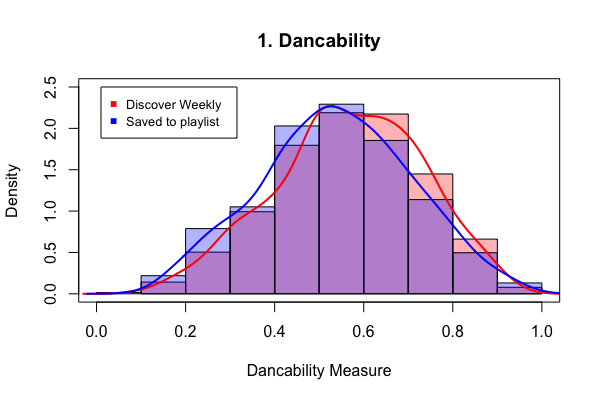
\includegraphics[width=\textwidth]{1_dancability} 
		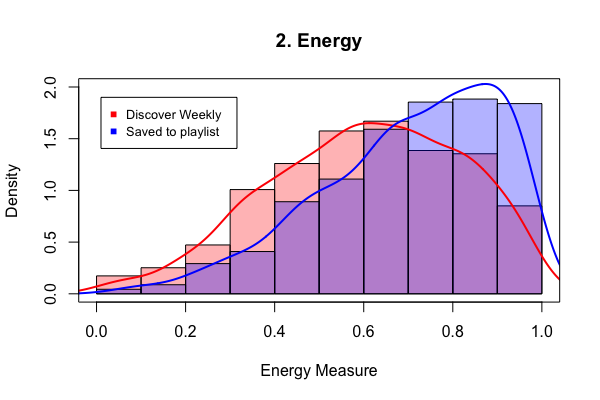
\includegraphics[width=\textwidth]{2_energy} \\
		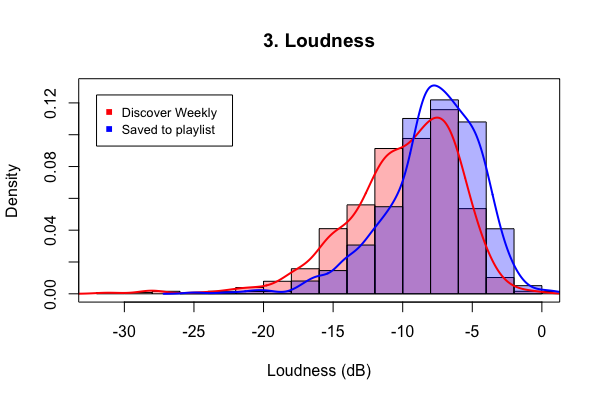
\includegraphics[width=\textwidth]{3_loudness}\\
		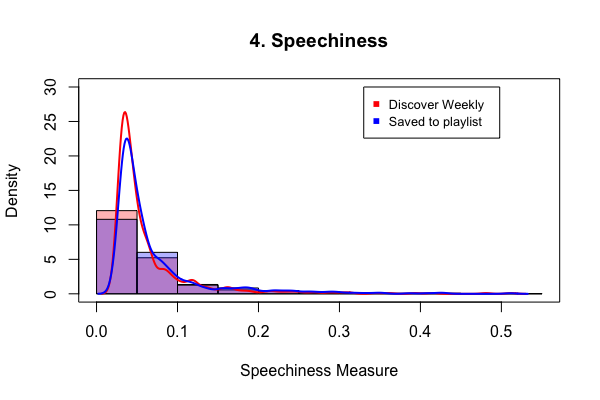
\includegraphics[width=\textwidth]{4_speechiness}\\
		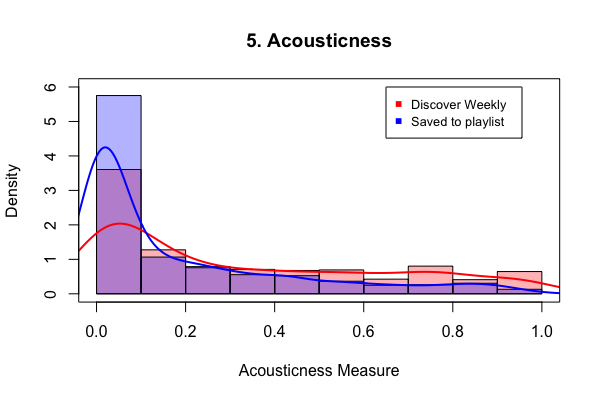
\includegraphics[width=\textwidth]{5_acousticness}\\
		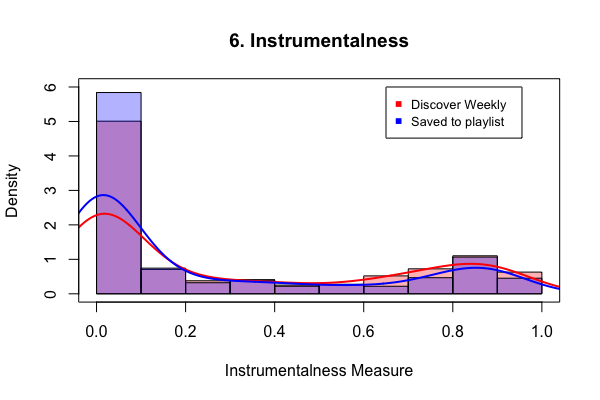
\includegraphics[width=\textwidth]{6_instrumentalness}\\
		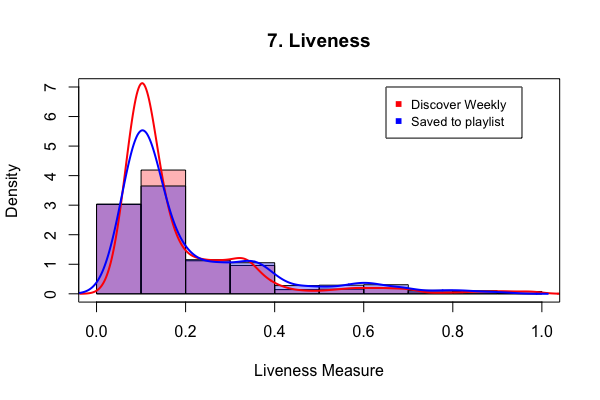
\includegraphics[width=\textwidth]{7_liveness}\\
		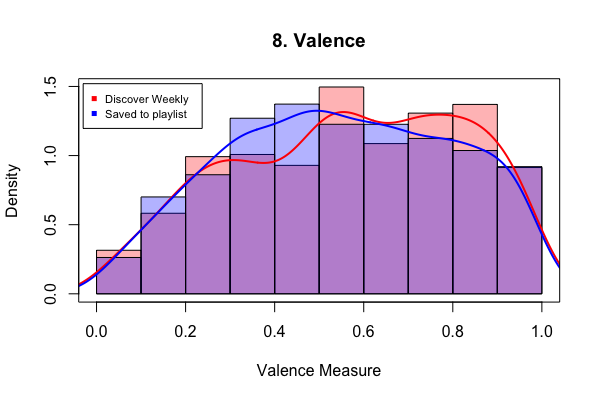
\includegraphics[width=\textwidth]{8_valence}\\
		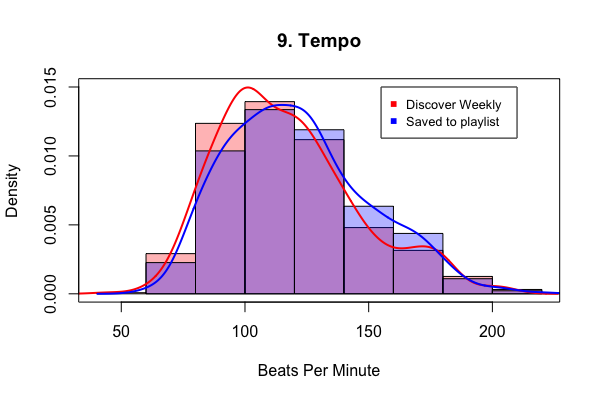
\includegraphics[width=\textwidth]{9_tempo}\\
		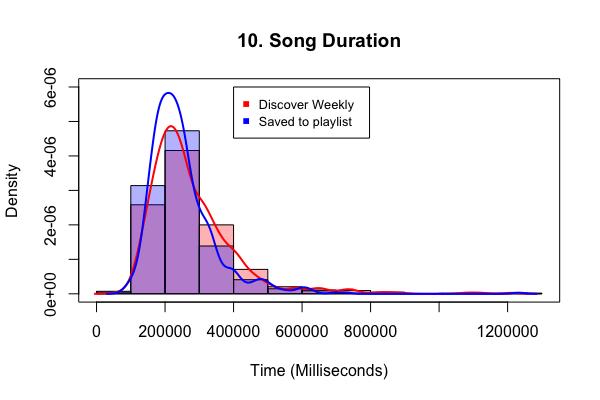
\includegraphics[width=\textwidth]{10_song_dur}\\
		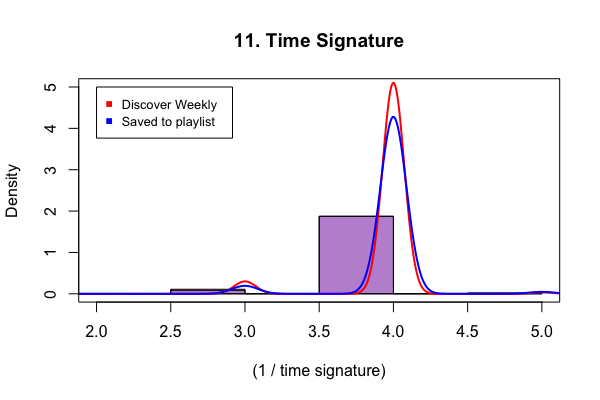
\includegraphics[width=\textwidth]{11_time_sig}\\
		
		As shown, Spotify (Red) tends to get my musical taste almost correct (Blue), but is just slightly off in a few areas. 
		
		\begin{enumerate}
			\item Danceability \\
				I tend to like more songs that have a medium danceability value (0.4-0.6), where Spotify thinks that I prefer songs that are more "dance-y".
			\item Energy \\
				Spotify tends to think that I have a slight preference towards songs with more energy, however this variable is the most seperation between my preferences and Spotify's predictions. A lot of the songs that I like have very high energy.
			\item Loudness
				I tend to like songs which are around the same loudness peak (-7.5dB), whereas spotify predicts I like songs that are over a wider spread.
			\item Speechiness
				Speechiness is used for describing spoken word, poetry, and a-capella performances. Spotify is correct in predicting that I do not listen to any of these performances on their platform.
			\item Acousticness
				I tend to not listen to acoustic performances, as shown by the majority of the distribution being spread over a small range around 0.1. Spotify tends to think that the range is more spread out, with a small peak around 0.8.
			\item Instrumentalness
				Spotify is pretty accurate with predicting the distribution of tracks that I listen to with instrumentalness measure (either not at all, or a few niche tracks).
			\item Liveness
				Again, Spotify has accurately predicted that I barely listen to songs that sound like a live recording.
			\item Valence
				This distribution is quite spread, however it is shown that Spotify's predictions tend to peak around higher valence values, whereas my preferences resemble more of a bell-curve distribution around 0.45.
			\item Tempo
				This tempo distribution follows the most common distribution of all songs available. 120BPM is the most common tempo for any modern western music, so therefore it is no surprise that the predicted values are similar to my saved favourite values.
			\item Duration
				Again, my saved favourites and popular songs tend to last the same amount of time (roughly 3 minutes), so Spotify is accurate in predicting this value.
			\item Time Signature
				Once again, the most common time signature is 4/4. Spotify correctly predicts the distribution of songs that I listen to with these time signatures. (If I listened to more prog-rock I could possibly skew this component...)
		\end{enumerate}
    
    \section{Machine Learning Methods}
    	As I would like to verify my hypothesis by using the accuracy of machine learning models, I have decided to use a variety of machine learning techniques to try and classify the dataset into the Discover Weekly set and Saved Favourites set. The assignment is formulated as a simple single value binary classification problem, and I want to verify similar results with different approaches, so I will not be using ANN style architectures. I will be using:
		
		\begin{itemize}
			\item Logistic Regression
			\item K-Nearest Neighbours
			\item Support Vector Machine (Linear Kernel)
			\item Support Vector Machine (Gaussian Kernel)
			\item Decision Tree
		\end{itemize}
		
		I believe that by spreading out the implementation of the classifiers onto these 5 methods will reduce the chance of having incorrect code, and will better support my original hypothesis that Spotify's Discover Weekly prediction is very good, but not perfect. I think that using a Neural Network Architecture would result in better results when classifying into the two sets, however it is not as easy to independently verify results with different techniques using ANN architectures.
		
		R implementation of experiments is included as "C1524413-part3-code.zip" and can also be found on GitHub\footnote{\url{https://github.com/harritaylor/discover-weekly-analysis}}, along with the original datasets.
	
	\section{Experimental Setup}
		I am running all experiments on a 2015 MacBook Pro Retina using RStudio, which has no issues running the proposed machine learning models. I am taking advantage of common machine learning libraries (including caTools, e1071, class, rpart, and ROCR) and techniques in order to make the development process as efficient as possible.
		
		Before constructing each classifier I am using a randomly sampled split to split the data into test and train sets, either with a split of 0.8 or 0.75. I am then using R's builtin scale() function to normalise the training set and test set independently, such that variables with large values do not skew the training.
		
		I am using the first 10 variables (the song features provided by Spotify) as independent variables, and "Saved" as the dependent variable to classify if the song should be saved to my personal favourites library based on the given song features. I am then using the RORC package to calculate the True Positive rate and False Positive rate for each model.

	\newpage
	\section{Results}
				
		\subsection{Logistic Regressor}
			I am constructing a logistic regression classifier using glm, with family set to binomial as the dependent variable is a yes/no classification. As the classifier outputs probabilities, I am using control flow statements to round the probabilities to either 0 or 1 in order to evaluate the regressor's predictions.

			
			\textbf{Accuracy}: 64.55\%

						
			\noindent
			\renewcommand\arraystretch{1.5}
			\setlength\tabcolsep{0pt}
			\begin{tabular}{c >{\bfseries}r @{\hspace{0.7em}}c @{\hspace{0.4em}}c @{\hspace{0.7em}}l}
  				\multirow{10}{*}{\parbox{1.1cm}{\bfseries\raggedleft actual\\ value}} & 
    				& \multicolumn{2}{c}{\bfseries Confusion Matrix} & \\
  				& & \bfseries p & \bfseries n & \bfseries total \\
  				& p$'$ & \MyBox{89} & \MyBox{70} & P$'$ \\[2.4em]
  				& n$'$ & \MyBox{47} & \MyBox{124} & N$'$ \\
  				& total & P & N &
			\end{tabular}

		\subsection{K-Nearest Neighbours}
		I am constructing a KNN classifier using knn, and giving the training and test set to train and validate on respectively. I am using a K of 32 as the rule of thumb is k should be the square root of the number of samples in the training set.
			
			\textbf{Accuracy}: 61.81\%

						
			\noindent
			\renewcommand\arraystretch{1.5}
			\setlength\tabcolsep{0pt}
			\begin{tabular}{c >{\bfseries}r @{\hspace{0.7em}}c @{\hspace{0.4em}}c @{\hspace{0.7em}}l}
  				\multirow{10}{*}{\parbox{1.1cm}{\bfseries\raggedleft actual\\ value}} & 
    				& \multicolumn{2}{c}{\bfseries Confusion Matrix} & \\
  				& & \bfseries p & \bfseries n & \bfseries total \\
  				& p$'$ & \MyBox{89} & \MyBox{70} & P$'$ \\[2.4em]
  				& n$'$ & \MyBox{56} & \MyBox{115} & N$'$ \\
  				& total & P & N &
			\end{tabular}
			
		\subsection{Linear Support Vector Machine}
			I am constructing a simple SVM as a concept using 'C-classification' as it is a classification problem, with a linear kernel to see if the data can be linearly separated.
			
			\textbf{Accuracy}: 65.53\%

						
			\noindent
			\renewcommand\arraystretch{1.5}
			\setlength\tabcolsep{0pt}
			\begin{tabular}{c >{\bfseries}r @{\hspace{0.7em}}c @{\hspace{0.4em}}c @{\hspace{0.7em}}l}
  				\multirow{10}{*}{\parbox{1.1cm}{\bfseries\raggedleft actual\\ value}} & 
    				& \multicolumn{2}{c}{\bfseries Confusion Matrix} & \\
  				& & \bfseries p & \bfseries n & \bfseries total \\
  				& p$'$ & \MyBox{67} & \MyBox{60} & P$'$ \\[2.4em]
  				& n$'$ & \MyBox{31} & \MyBox{106} & N$'$ \\
  				& total & P & N &
			\end{tabular}
		
		\subsection{Gaussian Kernel Support Vector Machine}
			This is a modified version of the previous SVM in order to see if exploring higher dimensional space yields better results.
			
			\textbf{Accuracy}: 58.79\%

						
			\noindent
			\renewcommand\arraystretch{1.5}
			\setlength\tabcolsep{0pt}
			\begin{tabular}{c >{\bfseries}r @{\hspace{0.7em}}c @{\hspace{0.4em}}c @{\hspace{0.7em}}l}
  				\multirow{10}{*}{\parbox{1.1cm}{\bfseries\raggedleft actual\\ value}} & 
    				& \multicolumn{2}{c}{\bfseries Confusion Matrix} & \\
  				& & \bfseries p & \bfseries n & \bfseries total \\
  				& p$'$ & \MyBox{75} & \MyBox{84} & P$'$ \\[2.4em]
  				& n$'$ & \MyBox{52} & \MyBox{119} & N$'$ \\
  				& total & P & N &
			\end{tabular}
			
		\newpage		
		\subsection{Decision Tree}
			Finally, I used a Decision Tree to see if this method yielded more positive results when classifying the dataset. However, the tree ended up being fairly balanced.
			
			\textbf{Accuracy}: 59.95\%

						
			\noindent
			\renewcommand\arraystretch{1.5}
			\setlength\tabcolsep{0pt}
			\begin{tabular}{c >{\bfseries}r @{\hspace{0.7em}}c @{\hspace{0.4em}}c @{\hspace{0.7em}}l}
  				\multirow{10}{*}{\parbox{1.1cm}{\bfseries\raggedleft actual\\ value}} & 
    				& \multicolumn{2}{c}{\bfseries Confusion Matrix} & \\
  				& & \bfseries p & \bfseries n & \bfseries total \\
  				& p$'$ & \MyBox{96} & \MyBox{95} & P$'$ \\[2.4em]
  				& n$'$ & \MyBox{64} & \MyBox{142} & N$'$ \\
  				& total & P & N &
			\end{tabular}
		\subsection{Performance Evaluation}
		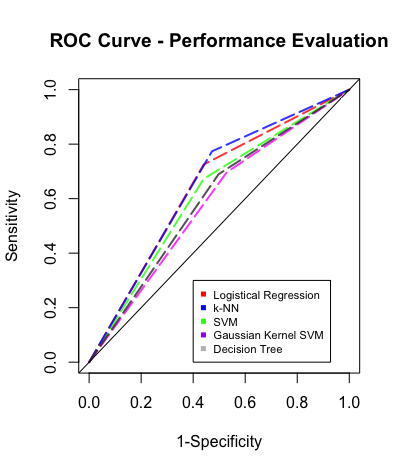
\includegraphics[width=\textwidth]{roc_curve} 
		
		As shown by the above ROC curve, all of the classifiers used for solving this classification problem have similar performance, which is to be expected. The classification problem is very difficult for machine learning techniques to solve with high accuracy as the two datasets are fundamentally very similar. The fact that average accuracy across the models is roughly 63\% mean that the models perform better than random guessing (685/1420 = 51\%).
				
		For future work I would attempt to classify the similar datasets using an ANN style machine learning technique such as deep learning. I would also increase the dimensionality of the variables to account for audio features as well as song features as this could provide a more insightful analysis, given the more powerful architecture.
		
			To answer the initial question, Spotify's Discover Weekly is a very good predictor of what kinds of songs I am likely to listen to. By comparing the generated and hand-curated playlists and resulting in a hard to classify problem proves that the datasets are fundamentally very similar. I am happy with the accuracy achieved by the models employed in this assignment, as it shows that there are relationships to be learned but the level of distinction between the two datasets is not high, leading to accurate recommendations from Spotify.
						 	
\end{document}
